\fancyhead[LO]{{\scriptsize {\FA \ }我们最幸福 {\FA } 好人命不长}}%奇數頁眉的左邊
\fancyhead[RO]{{\tiny{\textcolor{Gray}{\FA \ }}}\thepage}
\fancyhead[LE]{{\tiny{\textcolor{Gray}{\FA \ }}}\thepage}
\fancyhead[RE]{{\scriptsize {\FA \ }我们最幸福 {\FA } 好人命不长}}%偶數頁眉的右邊
\fancyfoot[LE,RO]{}
\fancyfoot[LO,CE]{}
\fancyfoot[CO,RE]{}
\chapter*{09 {\FA } 好人命不长}
\addcontentsline{toc}{chapter}{\hspace{5mm}09 \textbf{>}\ \ 好人命不长}
\vspace{15mm}
\begin{flushright}
	\textcolor{PinYinColor}{\EN \huge{The Good\\
	Die First\\
	\ \\}}
\end{flushright}

\begin{figure}[!htbp]
	\centering
	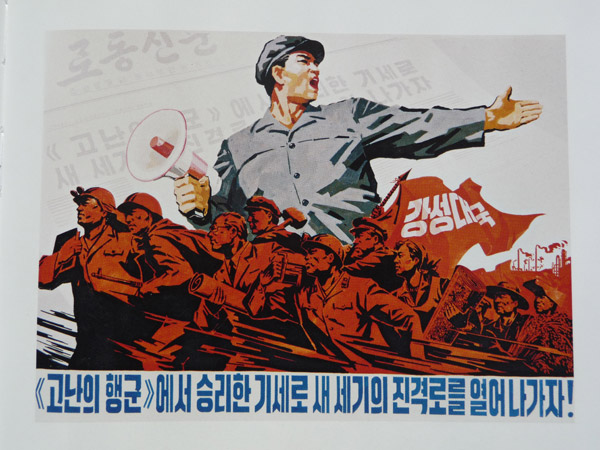
\includegraphics[width=6cm]{./Chapters/Images/09.jpg}
	\caption*{艰难行军的宣传画}
\end{figure}

\ifnum\theparacolNo=2
	\begin{multicols}{\theparacolNo}
\fi
据说在共产主义国家长大的人们无法自己谋生,因为他们习惯于政府无微不至的照顾。对于北朝鲜的饥民来说这不是真的。人们不甘心坐以待毙。当公共配给系统停止供应粮食后,人们为了生存想尽一切办法。人们用桶和细绳设置陷阱来扑捉野外的小动物,在阳台上,放置网兜抓麻雀。他们自己摸索一些植物的营养特性。他们回顾过去对饥荒的记忆,回忆父辈们对付饥荒的一些窍门。他们把带甜味的松树内层树皮撕成条,磨成细细的粉用于代替面粉。他们把橡子捣成一种胶状的糊,在用模子压成小方块,含在嘴里慢慢融化。\\

为了保命,北朝鲜人学会抛弃他们的尊严。他们在农业饲养的牲畜的粪便里捡拾那些没有被消化完的玉米粒。船厂的工人发明了新的技术,他们把堆放过食物的货船舱底部仔细的刮一遍,把刮出来的那些散发着恶臭黏糊糊的东西放在路边上晾干,然后从中收集没有煮过的米粒和其它可食用的东西。\\

在海滩上,人们从沙滩上挖着贝壳、采集海藻。在1995年的时候,当局沿着海边竖起了一道围栏\footnote{官方说是为防止间谍潜入,但是更可能的是阻止人们捕捉国营单位想控制的那些鱼类资源。},人们只好去海边那些没有防卫的峭壁用长长的耙子去收集海里的海藻。\\

没人告诉人们该怎么做──北朝鲜政府不愿意向外界承认粮食短缺──所以他们只好自己想办法。妇女们交流做饭心得。在制作玉米面时,不要丢掉玉米的壳、芯子、叶子和根茎,把这些都扔到磨子里。即便这些东西没有营养,也可以填饱肚子。面条至少煮上一个小时,这样看上去会更大些。找一些草叶放进汤里,以便看上去好像有蔬菜漂在里面。用松树皮粉做成糕。\\

收集和生产食物是所有人的重中之重。每天早上醒来要去找早饭,吃完早饭,你就要想晚饭怎么解决。午餐是属于过去的奢侈品。你可以在午餐时间睡觉,这样就可以保留体力。\\

然而,这还是不够。\\

在服装厂关门之后,宋女士内心挣扎着,彷徨着自己该干什么。她仍旧是个坚定的共产主义者,内心里憎恶腐朽的资本主义。她深深爱戴的伟大领袖金日成曾经反复告诫社会主义者必须“反对资本主义和修正主义恶毒的观点。”她喜欢引用这句语录。\\

然后,现实是自从伟大领袖去世,家里再也没有人领到过薪水──即使是她丈夫,一个党员及在电台有着一份如此体面的工作。长博再也得不到那些作为记者常有的免费葡萄酒和香烟作为额外津贴。宋女士明白是时候把自己的禁忌丢到一边,要去赚钱了。但是怎么才能赚到钱?\\

宋女士不太像个一般人眼里的生意人。她50岁,除了会用算盘算账,她没有什么其它的技能。当她同家里人发愁如何解决当前困境的时候,家人提醒她,她在厨艺方面的天赋。回到能得到食材的那些时候,宋女士很热衷于烹调,长博也很爱吃她做的美味。当然她的才能很自然也仅限于北朝鲜的风味,对外国的美食却没有尝试,但是即便如此,他们自己也很惊异的发现,虽然他们国家的名字现在几乎成了饥荒的代名词,但是北朝鲜的饮食文化之丰富也让人咋舌\footnote{实际上,南韩的很多餐饮业者都来自北朝鲜。}。北朝鲜的饮食很具创造性,通常使用天然食材,例如松茸和海藻。他们把当季的时鲜混合以大米、或者参杂玉米的大米,有时候加入当季的红豆酱或者辣椒粉。这道著名的菜式就是平壤冷面,其中冷的酸汤荞麦面根据地区不同也是千变万化,在加一个白水煮的鸡蛋、黄瓜或者梨。如果很忙,宋女士就会去商店买面条;如果有时间的话,她就会自己从淀粉开始做。利用从公共配给系统获得的一些的食材,她可以做炸菜,一种轻脆的油炸蔬菜。在她丈夫生日的时候,她就会用大米做香甜的糯米糕。她也知道如何做玉米酒。她的女儿们也常常夸耀她的泡菜是邻里间做的最好的。\\

家里人催促她在厨房里进行她第一次生意上的尝试,说最好的产品就是豆腐,在困难时期是一种蛋白质重要来源的食品。豆腐在朝鲜食谱中用处很广,可以用来做汤、焖煮、油炸或者发酵。宋女士用豆腐代替鱼,用油煎一煎再加上些红辣椒。为了筹钱买大豆,家里开始变卖他们的财产。第一件卖掉的就是家里引以为豪的日本产的电视机,那是为了表彰长博的父亲在朝鲜战争期间所做的情报工作而获得的奖励。\\

如果劳动力多,制作豆腐就相对比较简单。先把大豆煮一煮,然后磨碎,完了放入凝固剂。之后,就像奶酪一样,用一块布挤挤。再之后,就得到一些稀的豆奶和大豆壳。宋女士想了个好主意,她盘算用做完豆腐剩下的豆渣来养猪作为副业。而且公寓楼后面刚好有一排用来储物的大棚。宋女士在市场上买了些小猪,然后把他们安置在其中一个棚子里,并上了挂锁。\\

几个月下来,这门生意成功了。宋女士把她家小小的厨房变成豆腐作坊,把盛满大豆的大桶放在公寓里的炕炉上煮。由长博负责品尝并确认。小猪吃着豆渣、豆浆还有宋女士每天清晨外出割到的草长的也越来越肥。然而,要找到木头和煤炭烧炉子却越来越难了。电每周只来几个小时,即使这样,每家只能使用一个60瓦的灯泡,一台电视机或者收音机。没有燃料就没法煮大豆,宋女士也就做不成豆腐。没有豆腐,自然就没有豆渣喂那些猪。为了喂饱这些猪,宋女士每天要花好几个小时去割草。\\

“看来,我们自己可能也要吃草了。”她对长博打趣道。略有所思后接着说,“如果毒不死猪,也毒不死我们。”\\

于是,家里进入更严峻的新时期,他们再也不是那对曾自诩为美食家的有些身份的夫妇。宋女士每天都要从市中心向东、向西徒步步行很远的距离到那些地表没有被人工覆盖的地方,带着一把菜刀和一只篮子,沿途收集可以食用的野菜。如果走进山里,还可以找到即便在好辰光时人们也会吃的蒲公英和其它野菜。偶尔,宋女士会捡到一些农民扔掉的烂菜叶。她把白天捡到的东西拿回家,然后和其它买的起的任何食物混在一起。通常,就是些碎玉米面──一种很便宜的由玉米壳玉米芯磨成的粉。如果连这个都买不起,他就会买些更便宜的松树皮粉,有时候里面还会夹杂些锯末。\\

即使是表演天才也掩饰不了那种人憎鬼嫌的味道。她必须把野菜树皮切碎捣烂,弄成糊状,软软的才能下咽。这样的糊糊里没有多少东西,因此很难制成熟悉的面条状或者蛋糕状,虽然没什么分别,但是至少这些形状可以骗骗人,让他们以为是在吃真的食物。她现在能做的也就是这些没有什么味道,也没什么实质内容的粥。仅有的一点调味料就是盐。只要有一点大蒜或者红辣椒或许就能压住那可怕的味道,但是那些东西太贵了。食用油是有钱也买不到,没有油就很难做菜。有一次,宋女士去看望她姐姐的嫂子并被留饭,吃到的是豆秆和玉米芯做成的粥。即使那时候很饿,但是那一顿她简直咽不下去。又苦又干,卡在喉咙处,就像吞了一个鸟窝一样。她被噎住,脖子涨的彤红,最后还是吐了出来。她感觉受到莫大的侮辱。\\

在金日成死后的一年里,宋女士吃的唯一肉食就是青蛙。他在农村的兄弟抓了些。宋女士的嫂子把青蛙用酱油爆炒,然后切碎,和在面条里端上来。宋女士后来说那顿饭简直是美味啊。青蛙并不是朝鲜人的传统菜肴;宋女士以前也从来没吃过。不幸的是,这是她最后一次享用此等美味。到1995年,由于过度扑杀,北朝鲜的青蛙也几乎绝迹。\\

1995年年中,宋女士和她丈夫已经卖掉了家里大多值钱的东西换取食物。电视机之后就是他们主要的交通工具,日本产的自行车,也被卖掉了,接着是宋女士做衣服用的缝纫机。长博的手表和作为结婚礼物的一幅东方水彩画都被卖掉了。大多数的衣服和放衣服的大衣柜也都被卖掉了。曾经总认为很小的,容纳全家及家当的两居室公寓,现在看上去空空荡荡,除了墙上的金日成、金正日画像,真正的是家徒四壁了。省下能卖的就只有公寓本身了。\\

有个很奇怪的现象。在北朝鲜,你没用自己房子的产权;你仅仅是有居住在里面的权利。但是随着人们收买官员走后门暗地里交换住所,非法的房地产市场因此也出现了。宋女士经人介绍,认识了个妇女,她丈夫是曾在俄罗斯林场工作的北朝鲜工人,因此有些余钱想换一个更好的公寓。\\

宋女士的公寓的位置极佳,位于城市的中心地带,在没有公交车可以运行的时期就显得更为重要。宋女士和长博在这里住了20多年,在这里有很多的朋友。这也归功于她的性格,供职于人民班这么多年却一个仇人都没有。她和长博达成共识,他们不再需要这么大的房子。现在家里只有他们夫妇俩和长博的母亲。女儿们都出嫁了。儿子也搬去同那个年纪很大的,令宋女士很失望的女友同居,她只能想这样至少少了一张吃饭的嘴。\\

公寓换来了1万朝元──按照官方牌价合大概3000美元。他们搬到了一个一居室里。宋女士决定用手头的钱进行另外一次生意上的冒险:做大米生意。\\

大米是朝鲜人饮食中的主食。事实上,与大米(Baq)同一个字也有饭和食物的意思。1995年之后,清津的居民只能用现金在黑市上买到大米。咸镜北道的气候寒冷,多山的地形不适于种植稻米,只有靠近罗南的小水湾有些田地能种植水稻,所以这个城市所消费的大米大多靠火车或者卡车从外地运来,而道路、铁路路况都不佳,因此大米的价格也一直居高不下。宋女士盘算能南下从沿海地区低价收购些大米,然后坐火车运回来。交易大米或者其它类似的谷物,在北朝鲜都是很严重的违法行为\footnote{对当局而言,买卖蔬菜或其它食品相对来说还能容忍。},但是自从每个人都这么做之后,宋女士下决心冒这个险。这样,她可以赚点钱,还能给自己和长博留下些大米。想着这些,嘴巴竟然不由自主的流出口水。自1994年以来,他们家还没吃过一整碗的米饭。玉米只是大米的一半价格。\\

宋女士把1万块藏在内衣里,外面再罩几层冬衣。她坐上开往平安南道的火车,在那里买了大概200公斤的大米。在1995年11月25日的早晨,她踏上回家的路,其实也就是不到一天的路程,她把所买的大米堆放在自己的座位下面。长博利用自己记者的关系帮她弄到一张三等车厢的卧铺票。一等、二等车厢都是给劳动党干部及军官乘坐的。在当时那种情况下,宋女士对于自己享受的特权已是非常满意了。火车很长,每次转弯的时候都能看到后面长长的车厢,那里人们都没有座位,都站着。车厢里非常拥挤,只看见黑压压的一片。还有人爬到车顶坐着。在清晨8:30的时候,她刚刚爬下自己铺位,同包间里的其它乘客,一个军人、一个年轻妇女和一个老妈妈,聊着铁路糟糕的路况。整夜里,火车都走走停停,而且颠簸的非常厉害,以至于都没有办法吃早餐。他们的聊天也是断断续续的,每一次颠簸都会打断,直到一阵剧烈的颠簸把她震离座位,她重重的摔倒地板上,她的左脸撞到一个冰冷的东西上,后来才知道是窗户的金属框架。车厢整个侧翻了。\\

她听见后面的惨叫声。火车几乎扭成了麻花。后面拥挤的车厢几乎整个都毁了,大多数乘客都遇难了。而前面的车厢很幸运的幸免于难。至于这次发生于新浦,清津以南大概240公里处的事故到底死了多少人,有传言多达700人,但是正如其它北朝鲜的灾难一样,这次事故没有被公开的报导。\\

宋女士从车厢的残骸中慢慢爬了出来,脸颊上划了一道伤口,腿上也有块皮被扯掉了,背上也扭伤了。卧铺的床板落下来压住了她,但是因祸得福,可能也正是它的保护,她才幸免于难。在事故后四天,她才回到清津。她总是认为自己是个受幸运眷顾的人──在金日成的关爱下出生成长,有了个美满的家庭──从火车事故中死里逃生后,现在这个感觉就更尤为强烈。她疼得非常厉害,回到清津时,只能从火车上被抬下来,在站台上她看见长博,还有几个月没有讲话的儿子。看到他们,即使在事故中损失了大部分的大米,她仍然庆幸自己的好运。\\

宋女士受的伤其实她想象的来的严重的多。麻药过去了之后,她才意识到自己受的伤有多重。医生给了她一些止疼药,并叮嘱她要卧床休息3个月。但是她却将医嘱抛之脑后。要有人出去给全家找吃的。\\

在饥荒的时候,人们不都是饿死的。很多情况饥饿会先引发疾病。长期的营养不良会降低身体对抗病菌的免疫能力,而且饥饿让人们对结核,伤寒的抵抗力也逐渐丧失。饥饿使得人们非常虚弱,即使有抗生素,他们的身体也受不了,因此一点点可治愈的平常小病,突然就会使人们丧命。体内电解质等化学成分的剧烈波动也很容易引发中风、心脏病。人们也因为食用代食品而丧命,因为他们的身体消化不了那些东西。饥饿成为令人麻木的、飙升的儿童死亡率,或急剧降低的人口期望寿命的罪魁祸首。它导致了在此特定的情况下死亡率异常的情况──统计显示在此时期,死亡率高过正常数据。\\

死亡也有一个自然的过程。首先遭殃的是处于弱者的──5岁以下的孩子。他们先是患上感冒,进而恶化成肺炎;或是腹泻严重为痢疾。在父母们考虑求医问药的时候,可能孩子就已经死了。其次,死神盯上的就是老年人,从70岁的老年人开始,然后慢慢降至60岁甚至是50岁的人。这些人都会死,只是快慢的问题。之后,饥饿带来的死亡开始席卷青壮年。男人由于身体脂肪含量少往往先于女人死去。强健者及运动员也是死亡的重灾区,因为他们的身体新陈代谢旺盛因此也需要更多的热量维持生命。\\

然而更为残酷的是:死神光临的往往是最老实的,那些从来不偷、不骗、不坑、遵纪守法、不背叛朋友的人。正如意大利作家普里莫·莱维(Primo Levi)在奥斯维辛死里逃生之后,写道自己以及些那些幸存者之间在战后却不再想见面,因为他们所有人都做过见不得人,让人不齿的龌龊事情。\\

当宋女士10年后回首那些时日,当她想起清津那时候死的自己认识的人,她仅仅说了句“老实、善良的人、告诉他们做什么就做什么的听话的人──他们是第一批死的人。”\\

自己家里,宋女士的婆婆是第一个走的人。长博的母亲按照朝鲜传统,长子赡养父母的习俗,在他们结婚后不久就搬来和他们同住。照顾老人的责任也责无旁贷的落在了媳妇身上,因此朝鲜的媳妇和婆婆的关系总是不和的。宋女士的婆婆早年也是,常常对媳妇厉声斥责,特别是她生下了三个姑娘之后。仅仅是孙子出生后,她才有所改观,但是宋女士总是非常孝顺,也想方设法让老人开心。\\

春天在朝鲜是最为艰难的季节,因为秋天的收获快要耗尽而田里的下一季的庄稼才刚刚冒芽。而这一年,对从6个月前的事故中,刚刚恢复过来宋女士来说尤为艰难。她的婆婆现在73岁了,相对于北朝鲜人的平均寿命而言,已经是非常高寿了,因此也很容易让人认为她的去世是“时日到了”,但是宋女士却坚信这个凶巴巴的老太婆如果吃得好一些的话还能活很多年。由于不能做什么生意,也没办法到山里觅食,她把能在住所附近找到的野菜统统都扔进锅里煮汤。她婆婆也因此患上骨质酥松,眼睛周围也出现玉蜀黍疹。在1996年的5月,她吃坏了肚子,最后恶化成痢疾,几天后就去世了。\\

宋女士以一种朝鲜妇女可能的,最失败的方式没有尽到自己的责任。政府当局秋天里呼吁所有市民努力工作渡过难关的宣传,加上婆婆的死,使得她的绝望达到顶点。海报上,拿着扩音器的男人向人民疾呼“以胜利的精神在艰难行军中向新世纪前进”,他之后跟着戴钢盔的士兵、手拿铁镐的矿工、戴着眼镜,手拿蓝图的知识分子、戴着头巾的农民、还有拿着红旗的将军。即使是金正日,在官方报导里,在此期间也只吃些土豆做的简单食物。\\

现在只剩下夫妇两个了。宋女士和长博决定再次搬家,搬到个更小的地方。这次,仅比窝棚大一些,地板是水泥地面,墙面是斑驳的石膏墙面,脆的连金氏父子的画像都挂不住。她只好把画像仔细擦拭之后,放在墙角。他们没剩下些什么家当了。除了几本金日成、金正日写的书不能卖,她把长博其它的书都卖了。她还把她心爱的泡菜坛子也卖了。现在他们需要的只是两双筷子、两把汤勺、几个碗碟而已。\\

长博辞去了省电台的工作,到了铁路的一个广播站工作。铁路也没有钱付他工资──他们也仅仅是承诺在下一次食物配给时,给他更高的优先权。但是食物却从没发放过。几个月后,宋女士和她丈夫就花光了上次卖房子的钱。他们的大女儿玉熙,偶尔会从自家拿些玉米来,但是她要非常小心不被自己那脾气暴躁的丈夫发现,他会认为玉熙在“偷吃的”而揍她。他家里有些钱,但是却不愿意同自己的岳父母分享。\\

由于宋女士还不能到山里去寻觅,她只有起得更早,先是6点,之后5点就起来了,希望找到些隔夜长出来的野菜,这些野菜比较的嫩,也容易消化些。她会把野菜树皮煮的非常软,加点盐熬成粥再加几勺玉米面。\\

宋女士精疲力竭的时候反而觉得不饿那么了。在她吃完后,勺子就当的一声从手中滑落到金属盘子里。然后她就瘫在地板上,也不用麻烦去换衣服了,就这样昏沉沉的睡了,直到黑暗里,一种救生的本能告诉她是时候起来继续找吃的了。她现在没有任何意愿做其它的事情。她不再梳理她那曾引以为豪的卷发;她不再洗那些恼人的衣服。她的体重也下降的非常厉害,以至于单裤在她腰上就挂不住。她感到好像自己已经死了,好像魂魄飘出了曾是自己的身体的那副皮囊。\\

长博的健康状况也在恶化。他有着在北朝鲜人当中属于异乎寻常的高大身材,体重差不多90公斤。他实在太胖了,以至于几年前医生建议他尝试用吸烟来减肥。现在,他曾引以为豪的大肚子──在北朝鲜肥胖可是地位的象征──成了空心袋子。皮肤也成了鱼鳞状,貌似还得了严重的湿疹。他下颌下陷,说起话来含糊不清。宋女士一次送他去了铁路管理医院,在哪里,他被诊断是患了轻度中风;之后,长博发现他无法工作了。他不能集中注意力。他的视力开始减退,甚至连提笔写字的力气也没有了。\\

长博经常赖在床上或者躺着地板上他们仅剩的被子里。他的双腿像气球一样肿了起来,宋女士明白这是浮肿的症状──因为饥饿导致的水肿。他的话题也越来越多的围绕着食物展开。他说起童年时刻他母亲给他做的豆腐汤,还有他们新婚时宋女士给他做的异常美味的姜葱蒸蟹。甚至对宋女士十年前做的美味的每一个细节,他都有着异乎寻常的记忆力。当说起这些美味的时候,长博感概颇多,甚至还有些浪漫。此时,他握着宋女士的手,眼里闪着泪花,回忆这那些已经很模糊的记忆。\\

“来,亲爱的。让我们去好一点的馆子,再开一瓶红酒。”一天早上,当他们蜷缩在毯子里是,他告诉妻子。他们已经有3天滴米未进了。宋女士警惕的看着丈夫,担心他已经神志不清了。\\

宋女士全然不顾背上的伤痛,快步跑到市场上。她觉得去偷,去讨──总之不管用什么方法──给丈夫弄些吃的。她突然看见自己的姐姐在卖面条。他姐姐也好不到哪里去──由于缺乏营养,皮肤也和长博一样呈鱼鳞状──所以过去宋女士从不向她开口,但是今天顾不上了,当然,姐姐也不会拒绝。\\

“我会还给你的。”宋女士承诺着,带着面条跑回家,此时双腿完全靠着意志力驱动着。\\

长博在毯子下蜷缩成一团。宋女士喊着他的名字。但是他没有答应,她把他翻过来──因为长期挨饿,他体重降得非常厉害,以至于不费什么力气就把他翻了过来,但是此时的他手脚都已经僵硬了。\\

宋女士一遍又一遍的捶打着他的胸膛,大声呼救,即使她明白这一切都无济于事。\\

长博死后,他们的儿子,南玉搬回来和宋女士同住。自从他搬去和年长的女友同居后,母子就形同陌路了。实际上,宋女士同这个独子的关系,自儿子十几岁的时候就不怎么融洽。并不是南玉顽劣难以管教,而是她很难打破他的沉默。现在面临如此巨大的变故,那么与年长自己的女友同居的事实也就变得没那么重要了。而且更重要的是,他们需要相依为命。宋女士寡居,而南玉女友家的境况甚至还不如他自己家,她们家里也没有什么吃的了。\\

南玉的整个青少年期间都用于拳击训练,但是体校里的条件也非常差,所以在一个冬天冻坏了一只耳朵后,南玉回到了家中。他回了清津,通过家里在朝鲜战争中宋女士的父亲死于美国轰炸的这层关系,在火车站上找了一份工作。正如他的父亲一样,铁路管理局付不了南玉工资,只是解释在食品分配系统恢复运作时,可以他一些优先权。\\

宋女士的儿子很强壮,是个身材很好的年轻人,长得很像他父亲,只是更健壮,全身肌肉发达,身高175公分,在朝鲜人当中算很高的了。因此,他的生存也就需要更多的热量。刚开始的时候,是脂肪消失,他看上去精瘦的,像个马拉松运动员,但是后来,肌肉也消耗掉了,他几乎变成了一具皮包骨头的骷髅。在1997至1998年的冬天,气温降至冰点以下,他患上了严重的感冒,后来转成肺炎。即使瘦的不成形,但是要把他送去医院,对于宋女士来说,还是太重了。那个时候也根本没有救护车开的动。因此她只好一个人去医院向医生说明症状。一个医生给她写了处方,要打盘尼西林\footnote{即青霉素。},但是她去市场后发现,一支要50朝元,差不多是1公斤玉米的价格。\\

最后,她选择了玉米。\\

后来在1998年3月,南玉一个人孤独的死在那个小窝棚。那次,宋女士又一次跑到市场四处为他乞讨吃的。他后来在城北的一个小山头上被火化,同他的父亲葬在一起,那里离家很近,都能看见。铁路管理局也提供了个棺材,同长博一样的棺材。\\

截至1998年,估计有多达60万至200万的北朝鲜人死于饥饿或者由饥饿引发的病症,这几乎是总人口的10\%。在食品配给系统比其它地区更早中止的清津地区,死亡率甚至高达20\%。然而真实的数字似乎永远无法统计,因为北朝鲜医院写死亡报告的时候,是禁止用饥饿作为死因。\\

在1996至2005年间,北朝鲜总共接受多达24亿美元的粮食援助,而这些援助大多数来自美国。虽然北朝鲜当局愿意接受援助,但是它却拒绝外国人与之同行。试图提供帮助的援助机构的工作人员被严格限制在平壤和其它精心准备的地点。当他们被允许走出宾馆或办公室的时候,衣衫褴褛的人们都被驱离马路;在参观学校或者孤儿院的时候,只有穿的最好、吃的最好的孩子才会出现。政府一方面要求更多的援助,于此同时又把那些最需要帮助的人隐藏起来。居住在平壤的援助机构人员也不允许学习朝鲜语。\\

1997年,有些援助机构的官员被允许进入清津,在那里他们受到比在平壤更为严格的限制。曾为名为反饥饿行动(Action Against Hunger)的一个法国援助机构工作的工作人员在日记里写到,她不可以离开位于清津港附近的天马山宾馆,借口是她可能会被车撞到。这个机构不久就撤出了行动,因为他们不能保证救援能够抵达需要的人手中。随后,医生无国界组织(Doctors Without Borders)也撤出了。装载着联合国世界粮食计划署所捐助的谷物的巨轮于1998年开始在清津港卸货,此时,这些援助却被装上军队的卡车并被运走。有些食品最终到了孤儿院和幼儿园那里,但是更多的都被堆放进了军队的仓库,或者流向了黑市。联合国的相关机构花了差不多整整10年的时间才在北朝鲜建立起了一套令人满意的监督系统。到1998年底,饥荒最严重的阶段过去了,也不完全是因为各方面供应都在好转,宋女士后来推测,可能是要吃饭的嘴也少了很多。\\

“要死的人都死了。”\\
\ifnum\theparacolNo=2
	\end{multicols}
\fi